\chapter{时域积分方程基础}

时域积分方程(TDIE)方法作为分析瞬态电磁波动现象最主要的数值算法之一,
常用于求解均匀散射体和表面散射体的瞬态电磁散射问题。

\section{时域积分方程的类型}

\section{空间基函数与时间基函数}

利用数值算法求解时域积分方程,首先需要选取适当的空间基函数与时间基函数
对待求感应电流进行离散。

\subsection{空间基函数}

RWG基函数是定义在三角形单元上的最具代表性的基函数。它的具体定义如下:
\[ f_n(r) = \text{\ldots} \]
其中,$l_n$为三角形单元$T_n^+$和$T_n^-$公共边的长度,$A_n^+$和$A_n^-$
分别为三角形单元$T_n^+$和$T_n^-$的面积(如图~\ref{fig:rwg-demo} 所示)。

\begin{Figure}{fig:rwg-demo}{RWG基本函数几何参数示意图}
  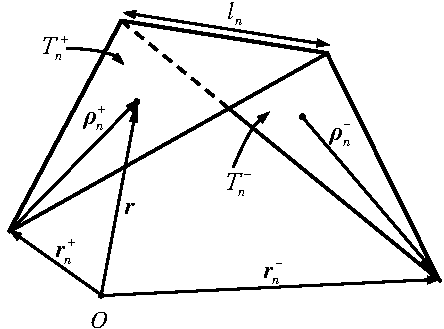
\includegraphics[width=0.5\textwidth]{ch/02/rwg-demo}
\end{Figure}

\subsection{时间基本函数}

\ldots

\subsubsection{时域方法特有的展开函数}

\ldots

\subsubsection{频域方法特有的展开函数}

\ldots

\subsection{入射波}

如图~\ref{fig:wave-a} 和图~\ref{fig:wave-b} 所示分别给出了参数\ldots

\begin{Figure}{fig:wave}{调制高斯脉冲时域与频率波形\\
      (a) 调制高斯脉冲时域波形;(b) 调制高斯脉冲频域波形}
  \subfloat[]{
    \label{fig:wave-a}
    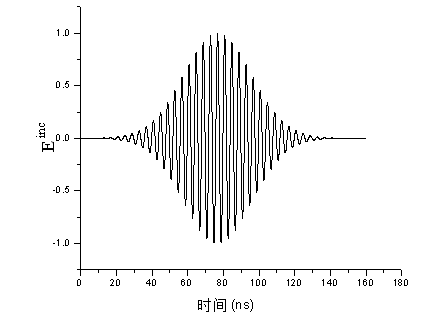
\includegraphics[width=0.4\textwidth]{ch/02/wave-a}}
  \subfloat[]{
    \label{fig:wave-b}
    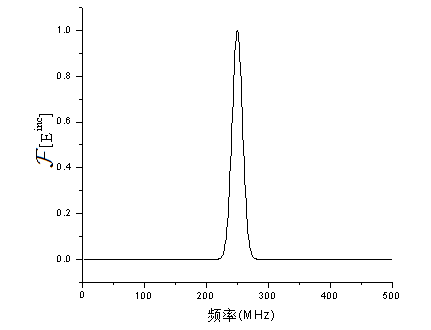
\includegraphics[width=0.4\textwidth]{ch/02/wave-b}}
  \captionsetup{margin={(\textwidth-\widthof{调制高斯脉冲时域与频率波形}-3em)/2,0em}}
\end{Figure}

\section{本章小结}

本章首先从时域麦克斯韦方程组出发推导得到了时域电场、磁场以及混合场积分方程。
